%%%%%%%%%%%%%%%%%%%%%%%%%%%%%% -*- Mode: Latex -*- %%%%%%%%%%%%%%%%%%%%%%%%%%%%
%%% ev_eval.tex --- 
%%% Author          : blehr
%%% Created On      : Thu Mar 11 05:41:23 1993
%%% Last Modified By: blehr
%%% Last Modified On: Sun Apr 11 13:41:38 1993
%%% RCS revision    : $Revision: 1.11 $ $Locker:  $
%%% Status          : In writing....
%%%%%%%%%%%%%%%%%%%%%%%%%%%%%%%%%%%%%%%%%%%%%%%%%%%%%%%%%%%%%%%%%%%%%%%%%%%%%%

\section{Evaluation}
\label{eval:eval}

As mentioned in Section~\ref{image:intro:categories}, the techniques
presented in Chapter~\ref{image} can be divided into two main
categories: {\em Noise reduction\/} schemes and {\em image
  segmentation\/} schemes.  With regard to the noise reduction schemes
presented in Section~\ref{image:noise}, it was pointed out there that
the presentation primarily was intended as an indicator towards some
possible techniques for removing noise from an image if it at a later
stage of the project should turn out that this would be necessary.
With that in mind, the noise reduction schemes are evaluated in
Section~\ref{eval:eval:noise}.

For the sake of clarity, the presentation of general image
segmentation schemes was divided in two: Image segmentation as a means
of recognizing parts of an image as belonging to a continuous region
with certain characteristics, elaborated upon in
Section~\ref{image:segment}; and edge detection, which was given
separate treatment in Section~\ref{image:edge}.  In
Section~\ref{eval:eval:segment} below, the image segmentation schemes
are evaluated, and in Section~\ref{eval:eval:edge}, the edge detection
schemes.  Note that the schemes are evaluated with respect to their
applicability fro detecting the pupil in an image, and that, when
evaluating them, it is assumed that the pupil is circular (cf.\
Section~\ref{back:eye}).

The key criterion for applicability is low computational cost.  In the
following, when comparing the computational cost of the different
techniques, it is assumed that the given image is of size $N\times N$,
and that the technique in question is carried out on the entire image.
The cost is measured in terms of $N$.  Obviously, the cost of any
technique applied on an entire image cannot be lower than $O(N^{2})$.
Thus, techniques are deemed too costly that are more expensive than
$O(N^{2})$.  Another obvious criterion is that the technique in
question serves the purpose.

\subsection{Noise Reduction Schemes}
\label{eval:eval:noise}

The noise reduction schemes presented in this chapter belong to two
different categories which are treated separately below: Spatial
domain and frequency domain schemes.

\subsubsection{Spatial Domain Approaches}

As pointed out in Section~\ref{image:spatial}, applying spatial
operators on an image generally requires $O(N^{2})$ operations.  Thus
the spatial noise reduction schemes presented in
Sections~\ref{image:noise:averaging} and~\ref{image:noise:median},
neighbourhood averaging, averaging of multiple images and median
filtering, perform in $O(N^{2})$ time.

Of the two averaging techniques, averaging of multiple images can be
discarded without delay, owing to its requiring several input images
of the same scene, a requirement which is unsustainable in our case.
Neighbourhood averaging has the drawback of attenuating the edges in
the image, thus making location of the pupil based on edge detecting
schemes difficult.

As pointed out in Section~\ref{image:noise:median}, median filtering
turns out to be clearly superior to averaging techniques, both with
respect to removing noise from an image and to maintaining edges in
the image.  In addition, median filtering is, when carefully
implemented, computationally cheaper than averaging schemes, in that
it requires mostly comparisons and no multiplications.

\subsubsection{Frequency Domain Approaches}

From Section~\ref{image:frequency:fourier}, p.~\pageref{pg:fft:O}, we
have that performing an {\fft} algorithm on an image requires
$O(N^{2}\log_{2}N)$ complex operations.  Thus image processing
techniques operating in the frequency plane generally perform in
minimum $O(N^{2}\log_{2}N)$ time, assuming that the image first has to
be Fourier transformed.  This applies to both simple highpass
filtering and selective filtering.

Simple highpass filtering has a similar effect to neighbourhood
averaging, namely blurring of the image, and consequently attenuating
of edges.  The selective filtering scheme would be better suited, but
then it is required to know the Fourier transform of the superimposed
noise function aforehand.  This is seldom the case in real-time
applications, where the noise normally has a random distribution.

The prohibitive aspect of these schemes (and of any frequency domain
scheme), however, is their computational cost, elaborated upon in
Section~\ref{image:frequency:fourier}, p.~\pageref{pg:fft:O}.  Thus
frequency domain noise reduction schemes implemented in software can
be discarded as an alternative in real-time applications (hardware
implementations may be fast enough to be sustainable).

\subsection{Pupil Detection Based on Image Segmentation}
\label{eval:eval:segment}

The term {\em image segmentation\/} refers in this section, as in
Section~\ref{image:segment}, to the problem of recognizing parts of an
image as belonging to a continuous region with certain
characteristics.  Edge detection schemes are treated separately in
Section~\ref{eval:eval:edge}.

\subsubsection{Thresholding}

As pointed out in Section~\ref{back:eye:visual}, the pupil constitutes
the darkest portion of the eye, and can thus be assumed to correspond
to the darkest region in an image of the eye.  Ideally, the
characteristics of a cross section of an image of the eye are as
depicted in Fig~\ref{fig:eye:cross:ideal}.  From this figure it is
evident that pixels belonging to the pupil by and large can be
recognized as such by thresholding the image with respect to a
threshold value $T$.

\insertpdf{crsideal}{\label{fig:eye:cross:ideal}An ideal cross
  section along the $x$ axis of an image of the eye.}

However, as pointed out in Section~\ref{image:segment:threshold}, the
problem with thresholding is, when applied to real images, to decide
on a value for $T$ which unambiguously differentiates between actual
pupil points and points not belonging to the pupil.  The probability
that all pixels in the pupil have values below $T$ and all pixels
outside of it have values above $T$ is for real images practically
zero.  Thus, in the most cases, applying a pure pixel-by-pixel
thresholding technique to obtain a binary image will on the one hand
result in an image where the pupil forms the largest recognizable
object; on the other hand, this object may have holes in it, and its
boundary will hardly form a perfect circle.

A better approach would be to apply some averaging technique in the
neighbourhood about the pixel to be thresholded, and then compare the
value returned to the threshold value $T$.  By carefully choosing the
averaging technique and equally carefully choosing $T$, it is possible
to design a {\em pixel filter\/} which only lets points through that
belong to the pupil.  Note, however, that it would only be possible to
design this filter so that no non-pupil points are let through; to
design it so that {\em all\/} actual pupil points are let through, is
for all practical purposes impossible.

From the above it can be concluded that thresholding is a technique
which enables the unambiguous recognition of a pupil point, although
as a means of reliably determining the {\em centre\/} of the pupil, it 
is not particularly suited.  Lastly, since thresholding is a spatial
technique, it performs in $O(N^{2})$ time.

\subsubsection{Region Growing}

Region growing is a technique which would seem well suited for
detecting the area and the extent of the pupil.  One problem, however,
is the requirement of a positive pupil point as seed point.  A search
algorithm operating on the image and employing a carefully designed
pixel filter of the kind depicted above as stop criterion could be
expected to return such a point.

Another problem is to chose the similarity criteria such that as many
actual pupil points as possible and as few non-pupil points as
possible are included.  A possible similarity criterion would be to
include those pixels whose values are below a given threshold value
$T$, assuming that the value of the seed point also is below $T$.
This would, however, result in exactly the same unsuitable pupil
region as the one supplied by the pixel-by-pixel thresholding scheme
above, given that the image and $T$ are the same.  A usual, and
better, similarity criterion is that the gray level of a pixel to be
included not differ from that of the seed point by more than a
specified amount.  This is, however, also a form of thresholding
(cf.\ Eq.~(\ref{eq:threshold:1}), p.~\pageref{eq:threshold:1}), and
puts a rigid limit on the interval of gray levels accepted.

Since the pupil is assumed to constitute the darkest region in the
image, having a relatively well defined edge to the surrounding iris,
a third approach would be to employ some sort of edge detecting scheme
(cf.\ Section~\ref{image:edge} as well as Section~\ref{eval:eval:edge}
below) as a criterion for inclusion.  That is, to use thresholding not
on the image itself, but on some sort of operator aimed at detecting
edges.  With this scheme, during the growing process, all pixels not
recognized as edge points are included.

The problems with this approach are to choose an optimal edge
detecting operator and, again, to choose an appropriate threshold
value $T$.  Also, the danger exists of the pupil having a boundary
with ``holes'' in it; that is, actual edge points that are not
recognized as such by the edge detecting operator.  In that case, the
region being grown will ``overflow'', i.e., it will cross the actual
boundaries of the pupil and possibly extend to include the entire
image.  By ensuring optimal illumination of the eye, in addition to
the care taken when choosing the edge detecting operator and the
threshold value $T$, it ought to be possible to reduce the probability
of this happening to a minimum.

After a region has been grown that corresponds as closely to the pupil
as possible, the problem remains of determining the position of the
{\em centre\/} of the pupil.  This can be done by, by means of some
data structure, registering the coordinates of the end points of the
rows and columns of the region being grown.  When the region is
complete, the $x$-position of its centre (and thus of the pupil's,
assuming that the correspondence between the region and the pupil is
approximately 1:1) is computed by taking the average of the centre
points of all rows (using the relation $x_{\mbox{\scriptsize
    centre}}=\frac{1}{2} (x_{\mbox{\scriptsize
    left}}+x_{\mbox{\scriptsize right}}$)).  The $y$-position is
computed analogously.

As mentioned above, region growing seems to suggest a reasonable
approach to the given problem.  It remains to be seen, however, if it
is computationally affordable in real-time applications.  In the
general case, that is, when the entire image is considered to consist
of contiguous regions that all are to be grown, region growing
performs in $O(N^{2})$ time with proportionality constant $1$.  In our
case, however, we are only interested in growing {\em one\/} region,
namely the pupil, and thus the proportionality constant depends on the
fraction of the image occupied by the pupil.  In our case, that is,
when the image covers the entire eye and no more, this fraction is
between 10\% and 20\%, thus reducing the proportionality constant to
between $0.1$ and $0.2$.  The number of operations required by the
algorithm searching for the seed point depends on the search strategy
employed.

\subsubsection{Template Matching}

As mentioned in Section~\ref{image:segment:template},~\cite{template}
offers an evaluation of three template matching algorithms for
detecting and locating the pupil in an image of the eye.  Of the three
match measures employed, the SAVD and the SSC are characterized as
satisfactory, whereas the correlation coefficient $\rho$ is deemed to
be ``inapplicable as a similarity measure''.

At any rate, due to its computational cost, software implemented
template matching can be discarded as an algorithm on which to base
the needed eye-tracking system.  To see why template matching is so
computationally expensive, consider once again Fig.~\ref{fig:template}
on p.~\pageref{fig:template}.  It is evident that the template has to
be moved to every pixel location in the image in order to obtain the
best match.  There are $N^{2}$ pixels in the image.  Assuming that the
template is of size $M\times M$, the number of operations required to
compute the match at any location is $O(M^{2})$.  Thus the total
number of operations is $O(M^{2}N^{2})$.  The diameter of the pupil in
a typical image of the eye is $\sim 0.3N$, yielding $M\approx 0.3N$.
This yields a total number of operations of $\sim 0.1N^{4}$, which
corresponds to template matching being $O(N^{4})$ in time!

\subsection{Pupil Detection Based on Edge Detection}
\label{eval:eval:edge}

All edge detection techniques presented in this chapter, except the
Hough transform, deliver images where the edges stand out on a
relatively uniform background.  The first technique described,
thresholding, returns a binary image where the edges detected are
emphasized.  For the latter two, gradient operators and highpass
filtering, a binary image can be obtained by appropriately
thresholding the returned image.  Thresholding and gradient operators
perform in $O(N^{2})$ time, whereas highpass filtering, as pointed out
in Section~\ref{eval:eval:noise}, performs in $O(N^{2}\log_{2}N)$
time.  The performance of the Hough transform is discussed below.

The main problem with determining the position of the pupil based on
edge detection is that it has to be known whether or not a given edge
corresponds to the contour between the pupil and the iris.  There is
nothing in the nature of this edge that uniquely separates it from the
other edges in the image.  There is, however, only one other circular
edge in the image, namely the iris-sclera edge.  By taking advantage
of the fact that the radius of the pupil only can take on values
within a certain interval, and that it always is smaller than the
radius of the iris, it would be possible to detect the pupil by
looking for an edge forming an circle whose radius lies inside this
interval.  This can be done by applying the Hough transform on the
image, as described below and in Section~\ref{image:edge:hough}.

Another way of unambiguously recognizing the pupil-iris edge as such,
is to make it the first edge that the edge detecting algorithm
encounters.  To ensure this, the edge detection procedure has to start
from a point positively classified as a pupil point, the {\em origin
  of operation\/}, and then carry on outwards in all directions until,
in each direction, an edge is detected.  All edges thus detected can
together be assumed to represent the pupil-iris contour.  By
registering the coordinates of opposite edge points, it is possible to
compute the position of the centre of the pupil, as described in the
previous section.  As a matter of fact, the last proposed inclusion
criterion for the region growing procedure---that only those pixels
that are {\em not\/} edge points be included---constitutes no more
than a concrete implementation of the algorithm described here.  To
supply the necessary pupil point, some search strategy can be applied
on the image, employing, for instance, a pixel filter, as described in
the previous section.

\begin{figure}[tb]
  \paragraph{}
  \makebox[0.425\textwidth][r]{
    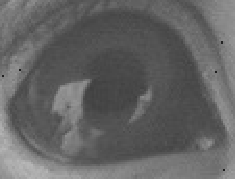
\includegraphics[width=0.3\textwidth]{figurer/monkbl05.pdf}}
  \makebox[0.45\textwidth][l]{
    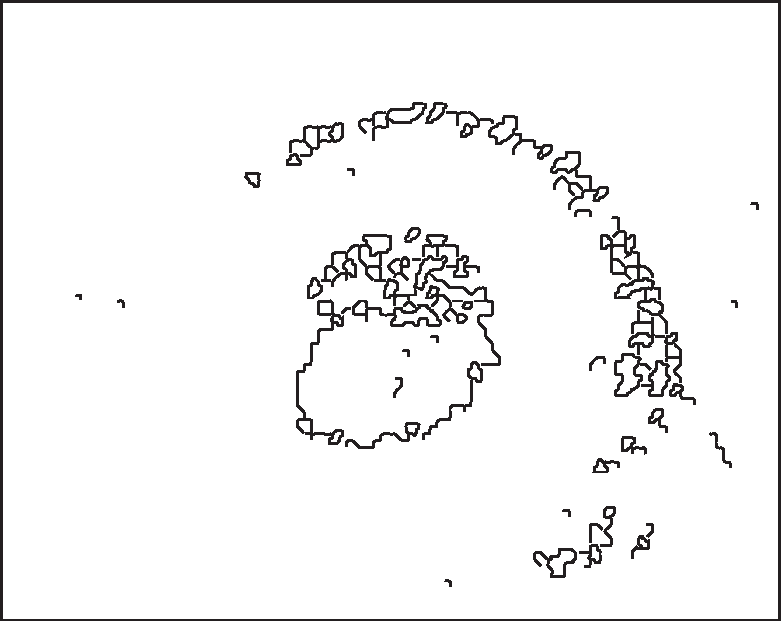
\includegraphics[width=0.285\textwidth]{figurer/threshld.pdf}}
  \hspace*{0.28\textwidth}(a)\hspace*{0.38\textwidth}(b)
  \paragraph{}
  \makebox[0.425\textwidth][r]{
    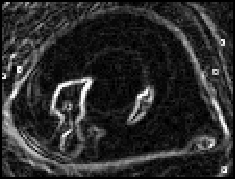
\includegraphics[width=0.3\textwidth]{figurer/soblbl05.pdf}}
  \makebox[0.45\textwidth][l]{
    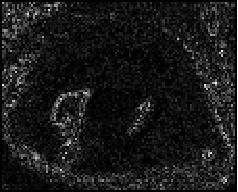
\includegraphics[width=0.285\textwidth]{figurer/laplbl05.pdf}}
  \hspace*{0.28\textwidth}(c)\hspace*{0.38\textwidth}(d)
  \caption{\label{fig:compare}(a) An image of a monkey's eye.  (b) The
    result of applying the thresholding procedure depicted in
    Section~\protect\ref{image:edge:threshold} on this image.  (c) The
    result of applying the Sobel operators on the image.  (d) The
    result of applying the Laplacian on the image.}
\end{figure}

The first three edge detection algorithms presented in
Section~\ref{image:edge}---thresholding, gradient operators and
highpass filtering---are evaluated with respect to being employed in
this algorithm.  The main evaluation criterion, next to computational
cost, is thus how strongly they respond to the pupil-iris contour. The
image in Fig.~\ref{fig:compare}(a) is used to illustrate the individual
responses of the techniques in question, except for highpass
filtering, for which no implementation has been made.  The Hough
transform is treated separately in the last part of the section.

\subsubsection{Thresholding}

Ideal step edges are seldom found in real applications, and neither
are edges that can be characterized by monotonously increasing or
decreasing functions.  Normally, an edge is characterized by a
function with spurious increases and decreases, but with an overall
tendency either to increase or decrease.  Thus the main problem with
the procedure described in Section~\ref{image:edge:threshold} is its
implicit requirement of having monotonous edges.  The ``bulb''-effect
of the procedure is clearly illustrated in Fig.~\ref{fig:compare}(b),
which can be viewed as a worst-case example; note in particular the
uppermost part of the pupil, where the actual edge has been
``drowned'' by spurious variations in gray level that lie on both
sides of the threshold value $T$.  This illustrates how critical the
choice of a value for $T$ is.

By choosing another value for $T$, it is clear that the result would
have looked different.  However, since the average gray level of the
images delivered by the camera tend to vary over time, it is not safe
to depend on a fixed threshold value in order to detect the pupil-iris
contour.  Moreover, this simplest form of thresholding looks only at
individual pixels, and accordingly induces no smoothing whatsoever,
leaving it too sensitive to noise.  All in all, thresholding can be
discarded as an edge detecting scheme applicable in the algorithm
described above.

\subsubsection{Gradient Operators}

As can be seen from the image in Fig.~\ref{fig:compare}(c), the Sobel
operators described in Section~\ref{image:edge:gradient} deliver an
image in which edges are depicted as relatively thick curves whose
intensities depend on the rate of change in gray level, as expected of
derivative operators.  The contour of the pupil is clearly seen,
although it is not very prominent.  The definitely strongest response
in the image is induced by the reflection to the left in the image,
where the largest transition in gray level takes place.  By carefully
choosing a threshold value for determining whether the response
corresponds to an edge point, it ought to be possible to employ the
Sobel operators in the above algorithm.  Note in particular that
gradient operators are insensitive to changes in the overall gray
level of an image.

In Fig.~\ref{fig:compare}(d), the result of applying the Laplacian on
the image in Fig.~\ref{fig:compare}(a) is shown.  As pointed out in
Section~\ref{image:edge:gradient}, the Laplacian does not respond as
strongly to edges as do other gradient operators.  Moreover, being a
second-order derivative operator, it tends to be unacceptably
sensitive to noise; note for instance the ``rippling'' in the upper
left corner of the image in the figure.  Most importantly, however,
and what excludes the Laplacian as a means of detecting the pupil, is
that the pupil is not discernible in the image at all.

\subsubsection{Highpass Filtering}

One prohibitive factor with respect to employing highpass filtering as
a means of detecting the edges of the pupil in our case, is the
computational cost of frequency domain methods in general, elaborated
upon in Section~\ref{image:frequency:fourier}, p.~\pageref{pg:fft:O}.
Moreover, as pointed out in Section~\ref{image:edge:highpass}, the
response given by highpass filtering schemes to edges in an image are
notably weaker than the response given by, for instance, first-order
derivative operators.  Lastly, it should be noted that, since noise
generally is high frequency in content, highpass filtering offers no
smoothing effect whatsoever, when applied to a noisy image.

\subsubsection{The Hough Transform}

As described in Section~\ref{image:edge:hough}, the Hough transform
can be employed to detect any curve or edge that can be described by
the equation $g(\vec{x},\vec{c})=0$, where $\vec{x}$ is a vector of
coordinates, and $\vec{c}$ is a vector of coefficients.  Thus, since a
circle is described by the equation
\begin{equation}
\label{eq:hough}
  (x-c_{1})^{2}+(y-c_{2})^{2}=c_{3}^{2}\mbox{,}
\end{equation}
the pupil can be detected by applying this equation in the Hough
transform.  The difference between the algorithm designed for
detecting lines, as depicted in Section~\ref{image:edge:hough}, and a
similar approach to detecting circles, is that the number of
parameters now is a triplet, $(c_{1},c_{2},c_{3})$, which results in a
three-dimensional parameter space, each coordinate triplet having an
accumulator cell associated with it.  Thus, for each accumulator cell
to contain the number of points in the image that lie on the circle
corresponding to it, both $c_{1}$ and $c_{2}$ are varied along their
respective axes, and and for each pair $(c_{1},c_{2})$,
Eq.~(\ref{eq:hough}) is solved with respect to $c_{3}$, the
accumulator cell associated with the triplet $(c_{1},c_{2},c_{3})$
being incremented for each solution.

In addition to having to deal with a three-dimensional parameter
space, it is evident from the relative complexity of
Eq.~(\ref{eq:hough}) that the application of the Hough transform to
detect circles in an image is rather expensive.  In
Section~\ref{image:edge:hough}, it was shown that the Hough transform
as applied to detecting lines in an image performs in $O(N^{2})$ time,
assuming that the proportionality constant $K$, corresponding to the
resolution along the $a$ and $b$ axes in parameter space, satisfies
the relation $K\ll N$.  In the three-dimensional case, however, the
proportionality constant is $K^{2}$, which makes it no longer sound to
assume $K^{2}\ll N$.  Moreover, due to high resolution in parameter
space being a prerequisite to high resolution in the $(x,y)$ plane, it
is more than probable that in our case $K$ would have to be chosen so
that $K^{2}>N$.  Consequently, the Hough transform as applied to
detecting the pupil in an image of the eye performs in $O(N^{2})$
time, but with a proportionality constant presumably larger than $N$.
Thus, also the Hough transform can be discarded as a suitable approach
to the problem at hand, on grounds on being too expensive
computationally.
